%
%%% FUNCTION
%
\section{関数,メソッド,サブルーチン}
\subsection{関数宣言}
\begin{frame}[containsverbatim,label=function,shrink]
\frametitle{関数,メソッド,サブルーチン}
  \begin{itemize}
\item 抽象化の方法について触れてきた
    \begin{itemize}
\item 変数: 計算の結果に名前をつけるということ
\item 配列: データの集まりを名前をつけて抽象化
    \end{itemize}
\item 今回は計算を合成する抽象化について見てみます
\item 合成したものに名前をつけて単一の手続きとして抽象化する方法
  \end{itemize}
\end{frame}
\begin{frame}[fragile,shrink]
\frametitle{Python における合成手続き}
  \begin{itemize}
\item Python では {\texttt def} というキーワードをつかって定義します
\item {\texttt def} のあとに関数名と仮引数を書いて,最後にコロン {\texttt :}(忘れずに)
\item 仮引数は関数を呼び出したときに実引数にバインドされる
\item 引数はその関数内だけで有効
  \end{itemize}
  \begin{columns}[t]
    \begin{column}{0.35\textwidth}
      \begin{lstlisting}[caption={add.py},label=lst:definefun]
a = int(input("a? "))
b = int(input("b? "))
wa = a
while b > 0:
  wa = wa + 1
  b = b - 1
print(wa)
      \end{lstlisting}
    \end{column}
    \begin{column}{0.3\textwidth}
      \begin{lstlisting}[caption={mult\_basicsonly.py},label=lst:definefun2]
def add(x,y):
  wa = x 
  while y > 0:
    wa = wa + 1
    y = y - 1
  return(wa)
      \end{lstlisting}
    \end{column}
    \begin{column}{0.3\textwidth}
      \begin{lstlisting}[caption={mult\_basicsonly.py},label=lst:definefun3,firstnumber=last]
def mult(x,y):
  seki = 0
  while y > 0:
    b = x
    seki = add(seki,b)
    y = y - 1
  return(seki)
      \end{lstlisting}
    \end{column}
  \end{columns}
\end{frame}
\subsection{計算の抽象化}
\begin{frame}[containsverbatim,shrink]
\frametitle{ブラックボックス抽象としての関数}
  \begin{itemize}
\item ``プログラムを部分に分ける''
\item どう分けるかが重要になる
\item 他のプログラムの部品として使え,まとまった仕事ができるようにわける
\item 部品としての関数はどう計算するかには関心をもたず,計算結果にだけ関心を持てば良い
  \end{itemize}
  \begin{columns}[t]
    \begin{column}{0.45\textwidth}
      \begin{lstlisting}[caption={bit\_string.py},label=lst:fun_abst]
### Set operations
def union(seta,setb,result):
  global Size
  for i in range(Size):
    result[i]=seta[i] or setb[i]
def intersection(seta,setb,result):
  global Size
  for i in range(Size):
    result[i]=seta[i] and setb[i]
      \end{lstlisting}
    \end{column}
    \begin{column}{0.45\textwidth}
      \begin{lstlisting}[caption={bit\_string.py},label=lst:fun_abst2,firstnumber=last]
def complement(seta,result):
  global Size
  for i in range(Size):
    result[i]= not seta[i]
def difference(seta,setb,result):
  global Size
  tmp=[-1]*Size
  for i in range(Size):
    complement(setb,tmp)
    intersection(seta,tmp,result)
      \end{lstlisting}
    \end{column}
  \end{columns}
\end{frame}
\begin{frame}[fragile]
\frametitle{仮引数と実引数}
  \begin{itemize}
\item 関数は仮引数というものをもつ
\item 複数の関数が同じ名前の仮引数を持っていても良い
\item 仮引数は関数の本体で有効である
\item 関数を呼び出したときの値に束縛 (bind) されて,関数の本体では呼び出し時の値に置き換えられる
\item 呼び出し時の値を実引数という
\item 一般に変数は有効範囲 (scope) が決まっている
\item 仮引数は関数本体が有効範囲である
  \end{itemize}
\end{frame}
%
%%% CRYPTOGRAPHY
%
\section{関数を使って世の中の事象を抽象化}
\subsection{暗号方式のおはなし}
\begin{frame}[fragile]
\frametitle{暗号通信}
  \begin{itemize}
\item 暗号システムを例に関数としての抽象化を見ていきます
  \end{itemize}
  \begin{center}
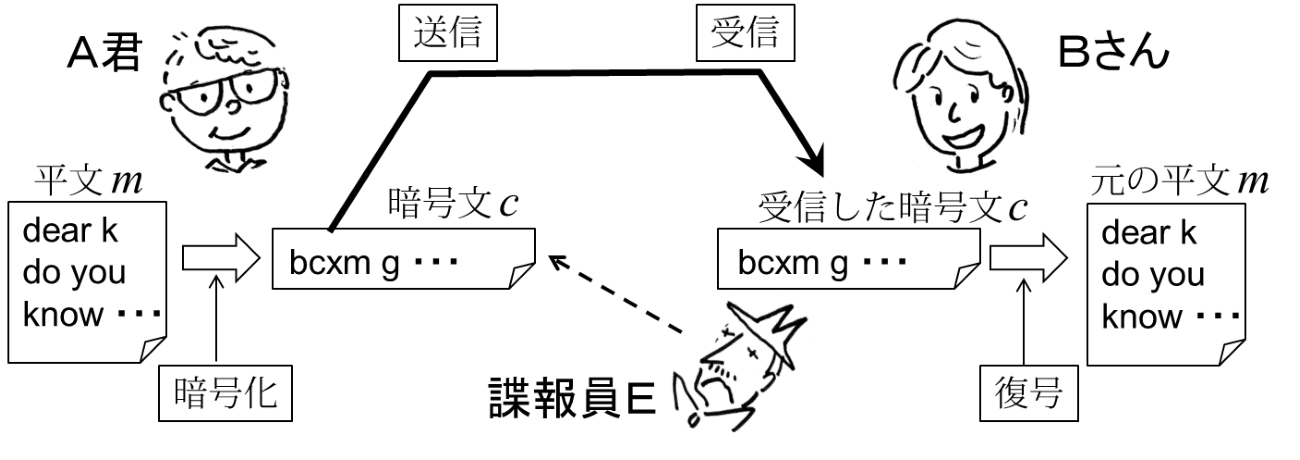
\includegraphics[scale=0.3]{./Figure/elementaryCS-figAliceBob.pdf}
  \end{center}
\end{frame}
\begin{frame}[fragile]
\frametitle{暗号方式 (Cryptography)}
  \begin{itemize}
\item シーザ暗号 (Caesar cipher): ローマ皇帝シーザが使った方式
\item ビジュネル暗号 (Vigen\`{e}re cipher): Vigen\`{e}re が作った方式
\item エニグマ (enigma): 大戦中にドイツ軍が使った方式
\item DES (Data Encyption Satandard), RSA (Rivest, Shamir and Adleman): 現在広く利用されている方式
  \end{itemize}
\end{frame}
\begin{frame}[fragile]
\frametitle{シーザ暗号}
  \begin{itemize}
\item 文字を $k$ 字先にシフトして暗号文を作る
\item \(k=3\) とすると下図のようになる
\item z, y, x は a, b, c になる
\item これからこれを関数として表していく
  \end{itemize}
  \begin{center}
    \begin{tabular}{ccccc}
a & b & c && z\\
$\downarrow$&$\downarrow$&$\downarrow$&$\cdots$&$\downarrow$\\
d & e & f && c
    \end{tabular}
  \end{center}
\end{frame}
\begin{frame}[fragile,shrink]
\frametitle{暗号システムに必要な要素}
  \begin{itemize}
\item $\cal M$: 文の集合
\item $\cal C$: 暗号文の集合
\item $\cal K$: 鍵の集合
\item \(\cal E\colon M\rightarrow C\): 暗号関数の集合
\item \(\cal D\colon C\rightarrow M\): 復号関数の集合
  \end{itemize}
  \begin{example}[Caesar Cipher]
\scriptsize
    \begin{itemize}
\item アルファベットは 0 から 25 に順番に対応付けられていると仮定する
\item $\cal M$: アルファベットの文字の列
\item $\cal C$: アルファベットの文字の列
\item $\cal K$: \(\{i\mid 0\leq i\leq 25\) であるような整数 $i\}$
\item \(\cal E\): \(\{E_k\mid k\in{\cal K}\ \mbox{and}\ \forall m(=m_1,m_2,\cdots)\in {\cal M}.E_k(m)=(m_i+k)\mod 26\}\)
\item \(\cal D\): \(\{D_k\mid k\in{\cal K}\ \mbox{and}\ \forall c(=c_1,c_2,\cdots)\in {\cal C}.D_k(k,c)=(26+c_i-k)\mod 26\}\)
    \end{itemize}
  \end{example}
\end{frame}
\begin{frame}
\frametitle{いくつかの用語}
  \begin{itemize}
\item \(E_k\in{\cal E}\) を \(m\in{\cal M}\) に適用することを暗号化 (encipher)
\item \(D_k\in{\cal D}\) を \(c\in{\cal C}\) に適用することを復号 (decipher)
\item \(k\in{\cal K}\) を 鍵 (key)
  \end{itemize}
  \begin{center}
    \begin{tabular}{ccc}
平文 (plaintext)&&暗号文 (ciphertext)\\
Hello World&$\stackrel{\mbox{暗号化}}{\rightarrow}$&Hhoor Wruog\\
Hello World&$\stackrel{\mbox{復号}}{\leftarrow}$&Hhoor Wruog
    \end{tabular}
  \end{center}
\end{frame}
\begin{frame}
\frametitle{シーザ暗号を関数であらわす}
  \begin{itemize}
\item 各文字を 0 から 25 で置き換える
    \begin{itemize}
\item a$\rightarrow$0, z$\rightarrow$25
    \end{itemize}
\item 暗号化関数 \(\mathit{enc}(3,m)=c\): 平文 \(m=m_1,m_2,\cdots,m_n\),暗号文 \(c=c_1,c_2,\cdots,c_n\) として \(f(m_i)=(m_i+3)\mod 26\) と表せる
\item 復号関数 \(\mathit{dec}(3,c)=m\): 平文 \(m=m_1,m_2,\cdots,m_n\),暗号文 \(c=c_1,c_2,\cdots,c_n\) として \(f^{-1}(c_i)=((26+c_i)-3)\mod 26\) と表せる
  \end{itemize}
  \begin{center}
    \begin{example}[Hello のシーザ暗号]
      \begin{itemize}
\item 暗号化は 関数 enc として enc(3,"Hello")="Hhoor" と表せる
\item 復号は 関数 dec として dec(3,"Hhoor")="Hello" と表せる
      \end{itemize}
    \end{example}
  \end{center}
\end{frame}
%
%%% CRYPTGRAPHY
%
\subsection{暗号通信のプログラム}
\begin{frame}[containsverbatim,shrink]
\frametitle{プログラムにしてみる}
\framesubtitle{宿題 4}
  \begin{itemize}
\item 関係として仕様をあらわしたので,実際にプログラムにしてみます
\item 具体的な計算として手続きを示した関数を定義します
\item 暗号システムという複雑なものを分割
  \end{itemize}
  \begin{lstlisting}[caption={ango.py},label=lst:ango]
# ango.py
# 暗号化サブルーチンの定義と利用
# 入力: 文字列
# 出力: 暗号化した文字列

### Global variables
K = 3 # 暗号鍵の設定

# 平文を暗号化するサブルーチン
# enc(秘密鍵 k, 平文 m) = 暗号文 c
def enc(k, m):
  ALPHABET = range(ord('a'), ord('z')+1) # 英字小文字アルファベット
  plain = list(m.encode("ascii"))        # 文字列 -> 文字コードの配列
  cipher = plain.copy()                  #暗号文格納用配列
  for i,code in enumerate(plain):
    ###
    # 宿題 4
    ###
  return(bytes(cipher).decode("ascii"))
  \end{lstlisting}
\end{frame}
\begin{frame}[containsverbatim,shrink]
\frametitle{宿題 4 (ango.py) のヒント}
  \begin{itemize}
\item \href{https://en.wikipedia.org/wiki/ASCII\#/media/File:US-ASCII\_code\_chart.png}{\beamerbutton{ASCII Code Chart}} を思い出してください
\item 小文字 a は 97 (0x61) が割り当てられています
\item アルファベットを 0 から 25 までの数字に対応づける
    \begin{itemize}
\item a の文字コード 97 を引くと文字を 0 から 25 に対応付けることができる
    \end{itemize}
\item {\tt m.encode("ascii")}で 1 バイトの文字コードの列に変換
\item {\tt list()} で配列を作成
\item 鍵 k 分だけ各整数にたす
\item 25 をこえるときは 0 にもどって計算
\item {\tt bytes(cipher).decode("ascii")}で文字の列に変換
  \end{itemize}
  \begin{center}
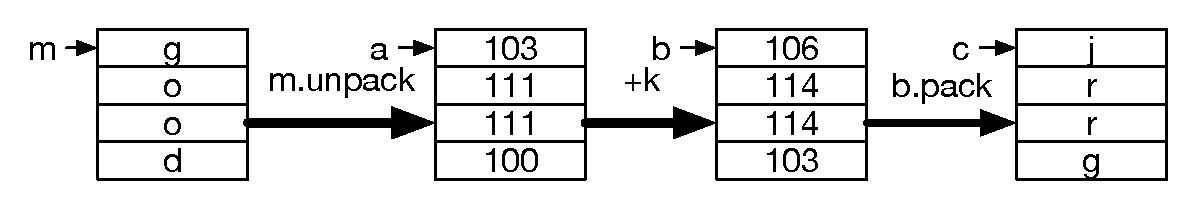
\includegraphics[scale=0.5]{./Figure/elementaryCS-figAngo.eps}
  \end{center}
\end{frame}
\begin{frame}[containsverbatim,shrink]
\frametitle{Python における文字列の操作}
  \begin{itemize}
\item {\tt str.encode("ascii")} で 1 バイトの列に変換
\item {\tt list()} で配列を作成
\item code.py を実行すると動作が見られます
  \end{itemize}
  \begin{lstlisting}[caption={code.py},label=lst:code]
# code.py
# 文字列処理の復習用
# 入力: 文字列
# 出力: 文字列の文字で小文字のみ,文字と各種情報を出力する
ALPHABET = range(ord('a'), ord('z')+1)         # 英字文字アルファベット
bun = input("Enter a string:")                 # 入力文字列から改行除法
cc  = list(bun.encode("ascii"))                # 文字列 → 文字コードの配列
for i, moji in enumerate(bun):                 # mojiはbunのi文字目を得る (i は 0 から始まる)
  code   = cc[i]                               # その文字のコードを得る
  offset = code - ALPHABET[0]                  # 文字 a との差分
  if code in ALPHABET:                         # 小文字アルファベットなら
    print(moji, ": ", code, ", ",hex(code), ", ", offset)   #   差分まで表示する
  else:                                        # そうでない時は
    print(moji, ": ", code, ", ",hex(code))    #   差分は表示しない
  \end{lstlisting}
\end{frame}
\begin{frame}[containsverbatim,shrink]
\frametitle{復号関数}
\framesubtitle{宿題 5}
  \begin{lstlisting}[caption={hukugo.py},label=lst:hukugo]
# hukugo.py
# 復号サブルーチンの定義と利用
# 入力: 暗号文の文字列
# 出力: 復号した平文
### Global variables
K = 3 # 暗号鍵の設定

# 平文を暗号化するサブルーチン
# dec(秘密鍵 k, 暗号文 c) = 平文 m
def dec(k, c):
  ALPHABET = range(ord('a'), ord('z')+1) # 英字小文字アルファベット
  cipher = list(c.encode("ascii"))       # 文字列 -> 文字コードの配列
  plain = cipher.copy()                   # 平文格納用配列
  for i,code in enumerate(cipher):
    ###
    # 宿題 5
    ###
  return(bytes(plain).decode("ascii"))
  \end{lstlisting}
\end{frame}
\begin{frame}[containsverbatim,shrink]
\frametitle{宿題 4, 5}
  \begin{itemize}
\item \href{https://sites.google.com/presystems.xyz/elementarycs/top}{\beamerbutton{https://sites.google.com/presystems.xyz/elementarycs/top}}から ango-skeleton.py と hukugo-skeleton.py をダウンロード
\item 同様にテスト用サンプルデータ plaintext.txt と ciphertext.txt をダウンロード(ソースコードと同じディレクトリに保存してください)
\item ファイル名は暗号化プログラム: ango.py, 復号プログラム: hukugo.py としてください
  \end{itemize}
\end{frame}
